\chapter{Week 06}

    The focus of this week was to integrate Gazebo into JupyterLab. The process involved four main steps: creating a new tab for Gazebo, building the website, displaying the website inside the created widget tab panel, and the consolidation with \texttt{jupyros}.

\section{Gazebo Extension I}

\subsection{Widget Tab Panel}

    By following the \href{https://github.com/jupyterlab/extension-examples/tree/master/widgets}{widget extension example} from JupyterLab, a new tab panel was created for Gazebo. With these modifications, the Gazebo tab can only be opened from the command palette. The appearance of the new panel is shown in Figure \ref{fig:widgetTab}. The background of the panel was adjusted in the \texttt{css} file for illustration purposes. 
    
    \begin{lstlisting}[language=TypeScript]
class GazeboWidget extends Widget {
  constructor() {
    super();
    this.addClass('gazebo-view');  // Used for css
    this.id = 'gazebo-widget';
    this.title.label = 'Gazebo';
    this.title.closable = true;
    \end{lstlisting}

    \begin{figure}[hb]
        \centering
        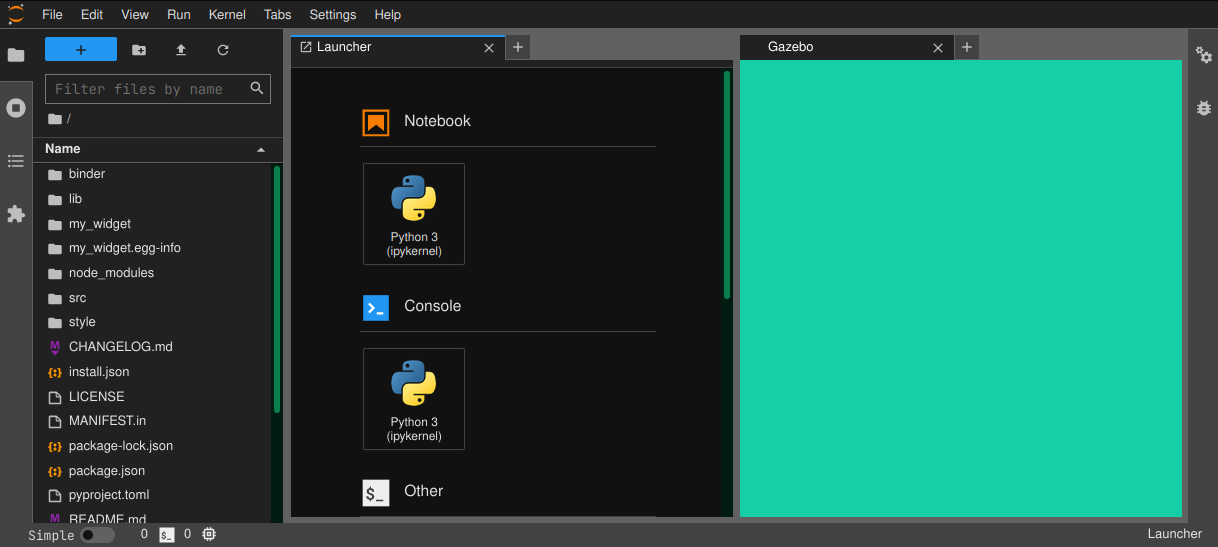
\includegraphics[width=0.95\linewidth]{Images/06_widgetTab.png}
        \caption{A Gazebo widget tab inside JupyterLab}
        \label{fig:widgetTab}
    \end{figure}
    

\subsection{Gazebo Website}

    Having previously built GzWeb, all the built files were simply copied and pasted into the \texttt{jupyterlab- gazebo} extension directory. The website displayed most of the components correctly in its new location with the exception of the model thumbnails once again. Although the thumbnails were in the correct folders, configuring the correct paths to the thumbnails required further investigation. 

% \begin{figure}[hb]
%     \centering
%     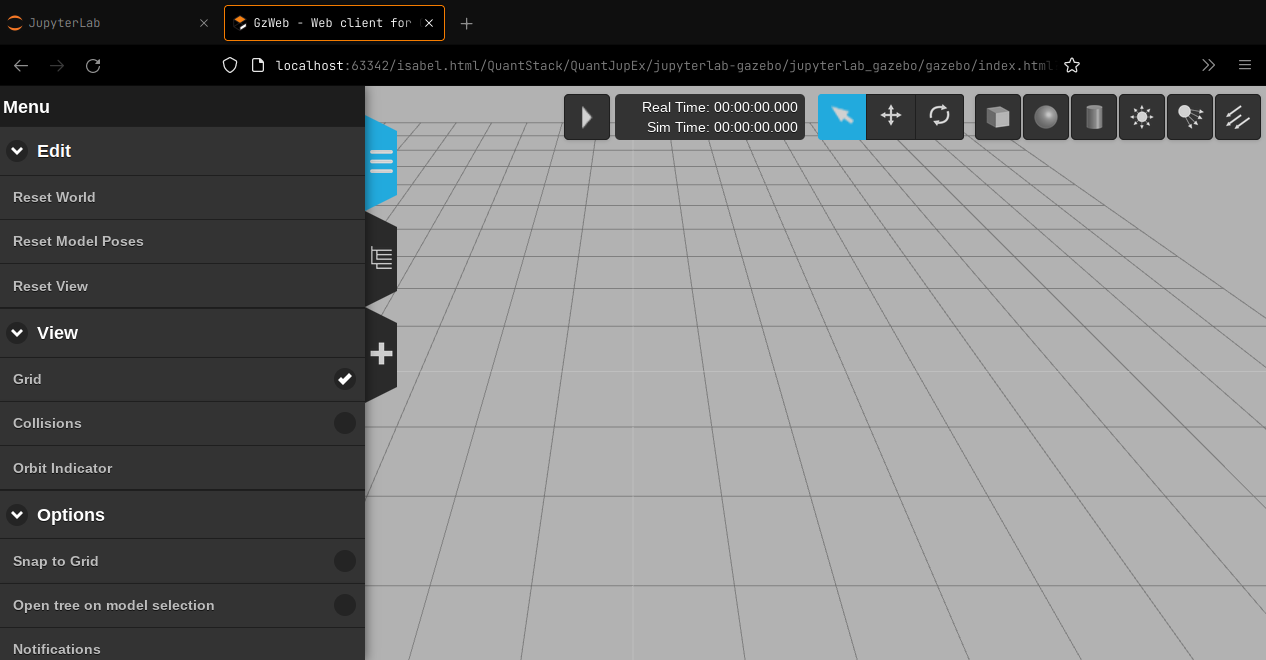
\includegraphics[width=\linewidth]{Images/06_gazeboTrial01.png}
%     \caption{Caption}
%     \label{fig:gzTrial1}
% \end{figure}

\subsection{Gazebo Widget}

    The next step consisted of putting the Gazebo website in an \texttt{IFrame} so that it could be displayed inside the tab panel. This step was mainly accomplished by following the configuration of Zethus. A new menu item was also included to make the opening and closing of the Gazebo view more easily accessible. Similar to Zethus, the URL for Gazebo was also configured so that the website could be accessed at \texttt{http://localhost:8888/gazebo/app/index.html}. The results can be observed in Figure \ref{fig:gzTrial2}.

\begin{figure}[h]
    \centering
    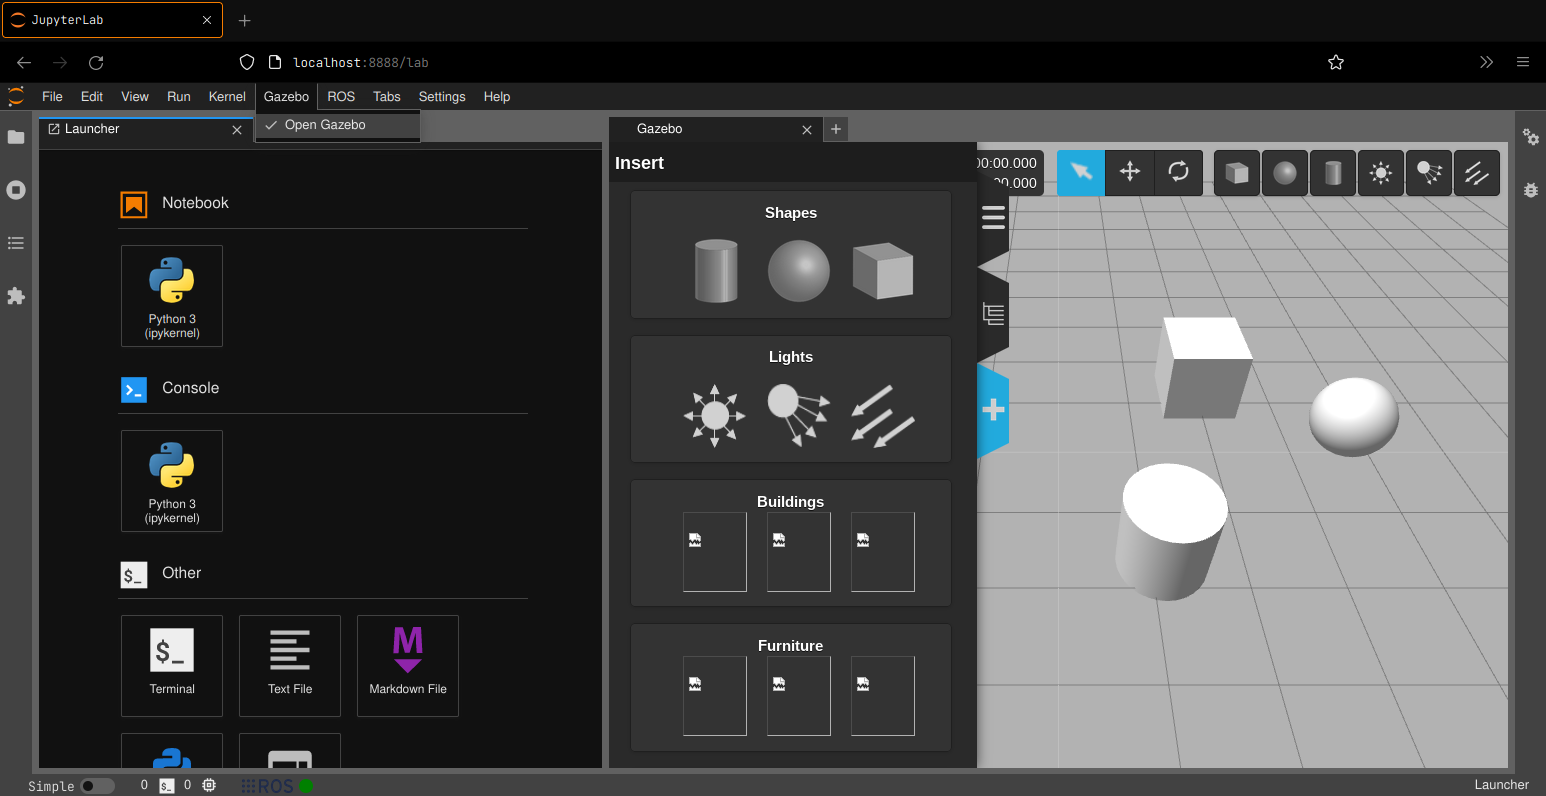
\includegraphics[width=\linewidth]{Images/06_gazeboTrial02.png}
    \caption{Display of Gazebo extension in JupyterLab}
    \label{fig:gzTrial2}
\end{figure}

\subsection{Integration with jupyros}

    Including the Gazebo widget as part of the \texttt{jupyros} tools required the simultaneous modification of the \texttt{jupyterlab-ros} package and the \texttt{jupyterlab-gazebo} extension. The \texttt{jupyterlab-ros} package creates the ROS menu and this is where a new list item needed to be added to open Gazebo as part of the ROS tools. And the Gazebo extension needed to be modified to reflect the change in the menu by removing the stand-alone Gazebo menu. 
    
    Although the idea was very simple, the execution was very involved. To begin, a new environment needed to be created where the Gazebo extension and \texttt{jupyterlab-ros} were in development mode. I also attempted to set \texttt{jupyter-ros} and \texttt{gzweb} in development mode within the same environment. Needless to say, no environment could be created which satisfied all the dependencies. Thus, the integration with \texttt{jupyros} remained pending.

\section{Future Work}

    Much work is left to be done to complete the Gazebo extension, this will include fixing the thumbnails issue, automating the build for GzWeb, and most importantly testing with ROS. Additonally, it would be a good idea to be able to export the ROS menu from the \texttt{jupyterlab-ros} extension to be able to add a new item from the Gazebo extension; this is in anticipation to future JupyterLab ROS extensions.
